\documentclass[11pt,letterpaper]{article}

\usepackage{subfigure}
\usepackage{graphicx}
\usepackage{amsmath}
\usepackage{amssymb}
\usepackage{enumitem}

\setlength{\textwidth}{6.5in}     
\setlength{\oddsidemargin}{0in}  
\setlength{\evensidemargin}{0in}
\setlength{\textheight}{8.5in} 
\setlength{\topmargin}{0in}   
\setlength{\headheight}{14pt} 
\setlength{\headsep}{10pt}   
%\setlength{\footskip}{0in}

%------------------------------------------------
\newcommand{\homework}[2]{
\setcounter{section}{#1}
\section*{ICS635 Homework {\thesection}: {#2} }
{\markboth{#2}{#2}}
}
%------------------------------------------------


\begin{document}

% Enter the Homework number and title as arguments to
% homework
\homework{1}{}

by: Lambert Leong\\ \\
\textbf{Problem 1}
\begin{enumerate}[labelindent=0pt]
\item 
	\begin{align*}
	E[aX+b] & = \int_{-\infty}^{\infty}(aX+b)f(x)dx \\
	& = \int_{-\infty}^{\infty}aXf(x)dx+ \int_{-\infty}^{\infty}bf(x)dx \\
	& = a\int_{-\infty}^{\infty} Xf(x)dx+b \int_{-\infty}^{\infty}f(x)dx \\
	& = aE[X]+b
	\end{align*}
\item 
	\begin{align*}
	var(cX) & = E[(cX - c\mu)^2] \\
	& = E[cX]^2 - (E[cX])^2 \\
	& = c^2E[X^2]-c^2(E[X])^2 \\
	& = c^2(E[X^2]-(E[X])^2) \\
	& = c^2(E[X]-(E[X])^2) \\
	& = c^2var(X)
	\end{align*}
\item 
	\begin{align*}
	var(x) & = \int_{-\infty}^{\infty}(x-\mu)^2f(x)dx \\
	& = \int_{-\infty}^{\infty}(x^2+\mu^2-2x\mu)f(x)dx \\
	& = \int_{-\infty}^{\infty}x^2f(x)f(x)+\mu^2 \int_{-\infty}^{\infty}f(x)dx-2\mu \int_{-\infty}^{\infty}xf(x)dx \\
	& = E[X^2]+\mu^2-2\mu^2 \\
	& = E[X^2]-\mu^2 \\
	& = E[X^2]-E[X]^2
	\end{align*}
\end{enumerate}

\noindent
\textbf{Problem 2}
\begin{enumerate}[labelindent=0pt]
\item 
	\begin{align*}
	E[X]  & = \int_{a}^{b}x(\tfrac{1}{b-a})dx \\
	      & = \tfrac{b+a}{2}
	\end{align*}
\item
	\begin{align*}
	var(X) & = E[X^2]-E^2[X] \\
	%& = E(x^2) - \mu^2
	& = \int_{a}^{b}\tfrac{x^2}{b-a}dx-(\tfrac{b-a}{2})^2 \\
	& = \frac{b^2+ba+a^2}{3} - (\tfrac{b+a}{2})^2 \\
	& = \frac{b^2-2ba+a^2}{12}
	\end{align*}
\end{enumerate}

\textbf{Problem 3}
\begin{enumerate}[labelindent=0pt]
\item 
%https://math.stackexchange.com/questions/786392/expectation-of-minimum-of-n-i-i-d-uniform-random-variables
%https://people.math.osu.edu/ban.1/532/min.pdf
	\begin{align*}
	F(x)=P(X\leq x)= 1 - P(X> x) = 1 - P(min(X_{1},X_{2})>x) \\
	\end{align*}
If $X_{1}$ and $X_{2}$ are evenly distributed on $[0,1]$ \\
	\begin{align*}
	F(x) &= 1-\left(\frac{b-x}{b-a} \right)^n = 1-\left (\frac{1-x}{1-0}  \right )^2 = 1-\left ( 1-x \right )^2 \\
	f(x) &= \frac{dF}{dx} = 2\left(-x+1\right) \\
	E[X] &= \int_{0}^{1}xf(x)dx = \int_{0}^{1}x2(-x+1)dx = \frac{1}{3}
	\end{align*}
%https://math.stackexchange.com/questions/105848/integrals-involving-minimum-function
\item
	\begin{align*}
	var(X) & = E[X^2]-E^2[X] \\
	& = \int_{0}^{1}x^22(-x^2+1)dx -\left ( \int_{0}^{1}x2(-x+1)dx
\right)^2\\
& = \frac{7}{45}
	\end{align*}
\item
	\begin{align*}
	cov(X,X_{1}) & = E[XX_{1}]-E[X]E[X_{1}]
	\end{align*}
%http://www.stat.ucla.edu/~rosario/classes/081/100a-2a/100aHW8Soln.pdf
\end{enumerate}

\textbf{Problem 4}
\begin{enumerate}[labelindent=0pt]
\item 
	\begin{align*}
	P(D|T^+) & =\tfrac{P(T^+|D)P(D)}{P(T^+)}
	\end{align*}
\item 
	\begin{align*}
	P(D|T^+) & =\tfrac{P(T^+|D)P(D)}{P(T^+)} \\
	& =\tfrac{P(T^+|D)P(D)}{[P(T^+|D)\times P(D)]+[P(T^+|not D)\times
P(not D)]} \\
	& = \tfrac{SP(D)}{[SP(D)]+[(1-Q)(1-P(D))]} \\
	& = \tfrac{.99(.001)}{[.99(.001)]+[(1-.99)(1-.001)]} \\
	& = .0902
	\end{align*}
\item 
	\begin{align*}
	P(D|T^+) & =\tfrac{P(T^+|D)P(D)}{P(T^+)} \\
	& =\tfrac{P(T^+|D)P(D)}{[P(T^+|D)\times P(D)]+[P(T^+|not D)\times
P(not D)]} \\
	& = \tfrac{SP(D)}{[SP(D)]+[(1-Q)(1-P(D))]} \\
	& = \tfrac{.99(.001)}{[.99(.001)]+[(1-.90)(1-.001)]} \\
	& = .0098
	\end{align*}
\end{enumerate}

\textbf{Problem 5}
\begin{enumerate}[labelindent=0pt]
\item 
	\begin{align*}
	\nabla f(x) &= \tfrac{1}{2}[\nabla x^TAx]+b^T \\
	\end{align*}
if A symmetric \\
	\begin{align*}
	\vec{\nabla} (x^TAx)=Ax+x^TA=2Ax \\
	\end{align*}
Then \\
	\begin{align*}
	&= \tfrac{1}{2}(2Ax)+b^Tx \\
	&= Ax+b^T
	\end{align*}
\item 
	\begin{align*}
	\nabla f(x) & = g(h(x)) \\
	& = g'(h(x))h'(x)
	\end{align*}

%chain rule?
% https://stats.stackexchange.com/questions/151066/gradient-of-loss-function-for-non-linear-prediction-functions
\item
	\begin{align*}
	{\nabla}^2f(x) &= \frac{1}{2}(x^TAx)=Ax+x^TA=2Ax = A \\
	\end{align*}
%\item
\item
	\begin{align*}
	\nabla f(x) & = \nabla g(a^Tx) \\
	& = g'(a^Tx)\nabla a^Tx \\
	& = (g'(a^Tx))a \\ 
	\end{align*}
	\begin{align*}
	\nabla ^2 f(x) & = \nabla (g'(a^Tx))a \\
	& = a^Tag''(a^Tx)
	\end{align*}
\end{enumerate}

\textbf{Problem 6}
\begin{enumerate}[labelindent=0pt]
\item
	\begin{enumerate}[labelindent=0pt]
	\item
	A small $\lambda$ would cause overfiting of the on the training set
and lead to low error.
	\item
	The overfit model will not generalize to the validation set well and
cause more error
	\item
	w will decrease
	\item
	The number of non-zero elemnts in w would be lower
	\end{enumerate}
\item
	\begin{enumerate}[labelindent=0pt]
	\item
	A big $\lambda$ could lead to under fitting on the training set which
would increase error
	\item 
	Underrfitting on the training set could lead to better generalization of
the validation set and reduce error.
	\item
	w magnitude will increase.
	\item
	There will be more non-zero elements of w.
	\end{enumerate}
\item
	\begin{enumerate}[labelindent=0pt]
	\item
	An L2 regularization encourages non-zero elements towards zero but they
dont actuall become zero.	
	\item
	\begin{align*}
	\nabla L & =   \sum_{n=1}^{N} \tfrac{\partial L}{\partial w} (y_{n}-(w^Tx_{n}))^2
\\
	& = \sum_{n=1}^{N}-2x_{n}(y_{n}-w^Tx_{n})
	\end{align*}
	\item
	\begin{align*}
	\nabla_{\theta}\mathcal{L}(\mathcal{D};\theta,\lambda) =   \sum_{n=1}^{N}
	\tfrac{\partial \mathcal{L}}{\partial w} (y_{n}-(w^Tx_{n}))^2 + \lambda
	||w||_{2}\\
	 =   \sum_{n=1}^{N} \tfrac{\partial \mathcal{L}}{\partial w}
	(y_{n}-(w^Tx_{n}))^2 + \lambda \sum_{d=1}^{D} \tfrac{\partial
	\mathcal{L}}{\partial w}w_{d}^2\\
	= \sum_{n=1}^{N}-2x_{n}(y-w^Tx_{n}) + \lambda \sum_{d=1}^{D} 2w_{d}
	\end{align*}
	\end{enumerate}
\end{enumerate}
\textbf{Problem 7}
\begin{enumerate}[labelindent=0pt]
\item 
The outcomes of the XOR functions are not linearly sperable.  Therefore, no
parameters exists that can lead to a zero loss for a single neuron.
\item
	\begin{align*}
	w_{1}^{(1)} & = 1,
	w_{2}^{(1)}  = 1, 
	b^{1}  = -.5 \\
	w_{1}^{(2)} & = -1,
	w_{1}^{(2)}  = -1,
	b^{2}  =1.5 \\
	w_{1}^{(3)} & = 1,
	w_{2}^{(3)}  = 1,
	b^{3}  = -1.5 \\ \\
	h_{1} &= (1*x_{1}+1*x_{2}+(-0.5)\\
	h_{2} &= (-1)*x_{1}+(-1)*x_{2}+(1.5)\\
	y &= (1*(h_{1})+(1)*(h_{2})+(-1.5)\\
	\end{align*}
\end{enumerate}

\textbf{Problem 8}
\begin{enumerate}[labelindent=0pt]
\item 
Feature scaling for linear classifiers will have little not no effect due to the
fact that weights are added to features and often times a bias term exists.
K-nearest neighbors (k-nn), on the other hand, measures the euclidean distance and will
be more affected by scaling. Scaling for k-nn would help to prevent a model from
being dominated by a feature with a large range. 
%https://stats.stackexchange.com/questions/249317/what-is-the-effect-of-data-scaling-when-compared-between-knn-naive-bayes-or-log
%https://stats.stackexchange.com/questions/244507/what-algorithms-need-feature-scaling-beside-from-svm
%https://stats.stackexchange.com/questions/121886/when-should-i-apply-feature-scaling-for-my-data
\item
The best accuracy for training and validation is 0.88 and 0.92 respectively.  The
income histogram indicated a lot of overlap between the two classes.  Also,
class 0 seemed to have some outliers.  Outliers were determined by x amount of
standard deviations (std) away from the mean.  While it is common to consider
data points outside of two std's from the mean to be an outlier, better training
and validation accuracies were seen when we excluded points that were outside of
1 std.

We used a K-nearest neighbors (Knn) model and experiemented with different
hyperparameters such as the algorithm used to compute the nearest neighbors,
weight function used in prediction, and the number of neighbors.  Ultimately,
the number of neighbors seemed to have the greatest effect on the accuracy.
\begin{figure}[h!]
        \centering
        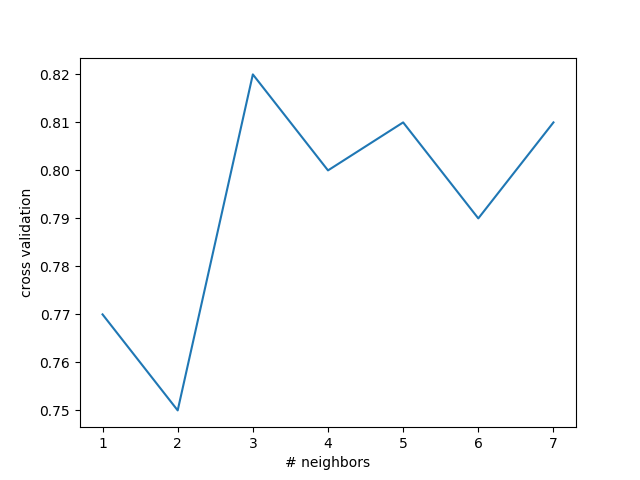
\includegraphics[width=.3\textwidth]{cv_plot.png}
        %\caption{Example of crossover. Viewing from the top the black solid
%vertical lines represent the center of mass.  Blue is associated with parent 1
%and red is associated with parent 2.}
        \label{fig:crossover}
\end{figure}
\item
The number of neighbors is the hyperparameter I chose to optimize.  It appears
that it is best to used an odd number of neighbors.  Three neighbors lead to the
best cross validation accuracy.  Any more and any less seem to yeild lower
accuracies.  


\end{enumerate}

\noindent\end{document}
